% SudokuScan - COMP 482 Project 1 report
% Compiles with IEEEtran (e.g. on Overleaf). If IEEEtran.cls is not
% installed, it falls back to a two-column article layout.
\IfFileExists{IEEEtran.cls}{%
  \documentclass[conference]{IEEEtran}%
  \def\usingieee{1}%
}{%
  \documentclass[10pt,twocolumn,a4paper]{article}%
  \usepackage[margin=1.8cm,columnsep=0.6cm]{geometry}%
  \usepackage{mathptmx}%
  \usepackage[font=small]{caption}%
}
\usepackage{graphicx}
\usepackage{booktabs}
\usepackage{amsmath,amssymb}
\usepackage{multirow}
\usepackage{stfloats}
\usepackage[hidelinks]{hyperref}
\graphicspath{{figs/}}
\usepackage{xcolor}

% ---- numbers from the held-out synthetic set (filled in from analysis/) ----
\newcommand{\SYNCORNER}{0.38}
\newcommand{\SYNACC}{99.3}
\newcommand{\SYNFONE}{0.991}
\newcommand{\SYNEXACT}{90.0}
\newcommand{\SYNROB}{100}

% ---- Appendix C entries (student reviewed) ----
\newcommand{\todo}[1]{\textcolor{red}{[#1]}}
\newcommand{\STUDENTKEPT}{I read the code and ran it on my 13 photos. I checked
the outputs and the debug images.}
\newcommand{\STUDENTREPORT}{I read the draft and checked the numbers with my
results.}
\newcommand{\STUDENTOWN}{and checking the results}
\title{SudokuScan: From a Phone Photograph of a Printed Sudoku to a Digital Grid}
\author{Furkan Can (042301138)\\COMP 482 Computer Vision, MEF University}
\date{5 November 2026 (revised 6 November 2026)}

\begin{document}
\maketitle

\begin{abstract}
SudokuScan reads a printed sudoku from a phone photograph. It finds the four
outer puzzle corners with the Harris detector, rectifies the puzzle with an
affine (3 and 4 point) and a projective model, recognises the givens with
Tesseract and checks them against the sudoku rules. On a personal dataset of 13
annotated photographs (three puzzles, conditions C1--C5) the system reaches a
mean corner error of 0.71\% of the puzzle side, 99.9\% cell accuracy, an
empty-cell F1 of 1.000 and 100\% robustness. The affine models are acceptable
only for near-frontal views (obliqueness below about 0.05); beyond that the
homography is required.
\end{abstract}

%=====================================================================
\section{Introduction}
The input is a single phone photograph of a printed sudoku; the output is
(a) the four outer corners (TL, TR, BR, BL), (b) three rectified
$450\times450$ images (A3, A4, H4), (c) the $9\times9$ grid of givens and
(d) a validity verdict. The problem is hard because the photographs are taken
from oblique viewpoints (perspective distortion), the page may be rotated,
lighting is uneven, and the background contains text, objects and other
rectangles that also produce strong corners.

The pipeline has six stages: illumination-normalising preprocessing, Harris
corner detection with a region-restricted extreme-point selection rule,
rectification with A3/A4/H4, an affine-versus-homography comparison,
cell extraction with an explicit empty-cell rule and Tesseract OCR, and a
validity check. All kernel sizes are fractions of the image width; large
photographs are reduced to 1000\,px for corner detection and the corners are
mapped back to original pixels. Bonus parts B1--B4 (solver, AR overlay,
many-point homography, any orientation) are implemented.

%=====================================================================
\section{Corner detection}
\subsection{Preprocessing}
The image is converted to greyscale and blurred (kernel $0.003w$). Uneven
illumination is removed by dividing by a background estimate: a
morphological closing with a $0.04w$ elliptical kernel removes thin dark
structures (lines, digits) and leaves the paper brightness, including
shadows. An adaptive threshold (block $0.025w$) gives a binary image.

\subsection{Harris response and candidates}
\texttt{cv2.cornerHarris} is run on the normalised image with
\texttt{blockSize} $=0.004w$ ($\approx4$\,px), \texttt{ksize} $=3$ and
$k=0.04$. Candidates are pixels with $R>0.01\max R$ that are the maximum of
their $(2r+1)^2$ neighbourhood (non-maximum suppression via
\texttt{cv2.dilate}). The NMS radius $r$ is 1\% of the puzzle side, not of the
image width: with an image-relative radius, a strong digit stroke next to the
outer corner of a small puzzle suppressed the corner itself (corner error
3.5\% on a synthetic test image, 0.22\% after the change). A typical photograph
gives about 330 candidates (Fig.~\ref{fig:harris}).

\begin{figure}[t]
\centering
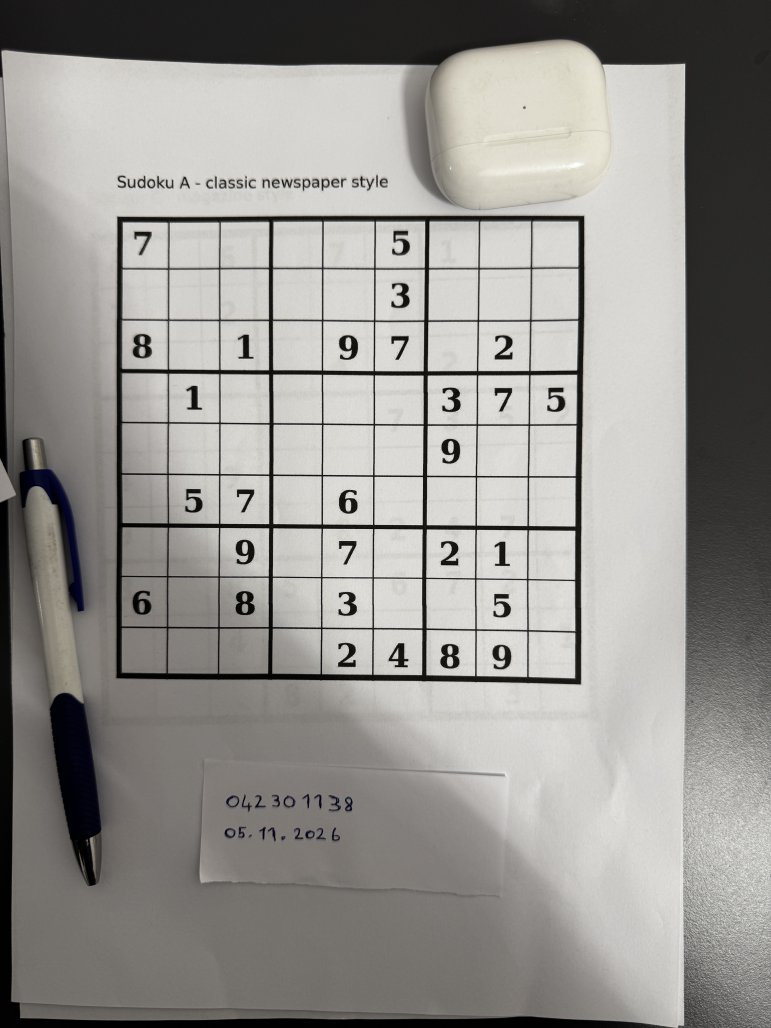
\includegraphics[width=0.48\linewidth]{IMG_0847_small.jpg}\hfill
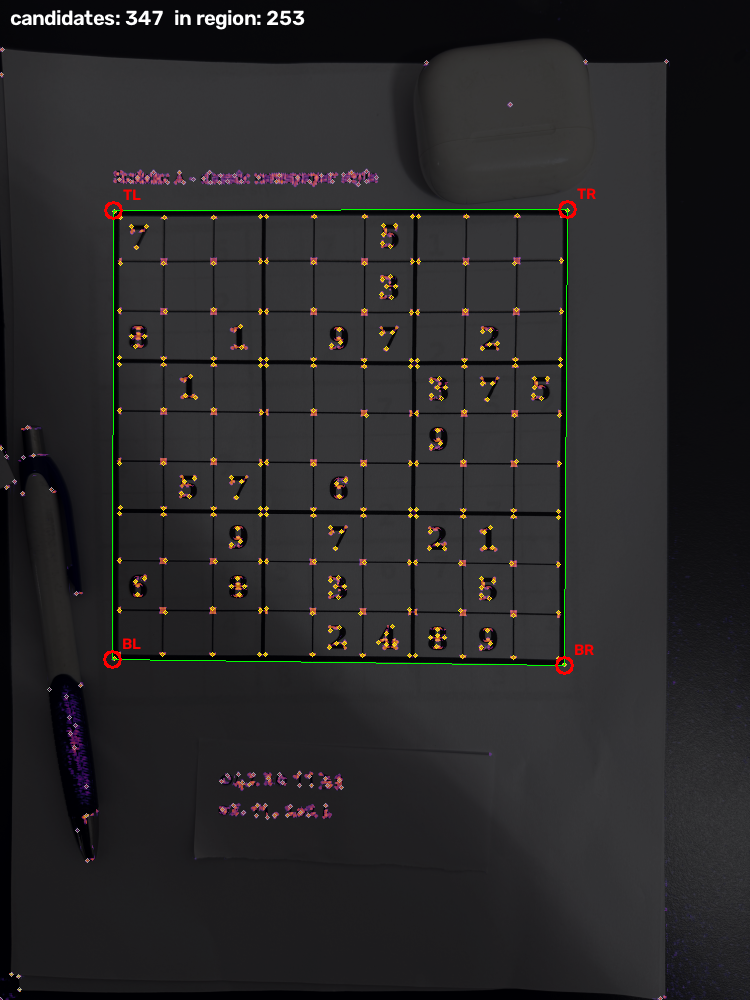
\includegraphics[width=0.48\linewidth,trim=150 0 150 0,clip]{harris_0847.png}
\caption{C5 example (IMG\_0847, earphone case, pen, show-through text).
Right: Harris response (log scale), all candidates (grey), candidates inside
the puzzle region (yellow) and the four selected corners (red).}
\label{fig:harris}
\end{figure}

\subsection{Corner-selection rule}
\begin{enumerate}
\item \emph{Puzzle region.} I first find contours and use their convex hulls
to identify quadrilateral candidates that cover at least 2\% of the image
area. I warp each candidate into a $180\times180$ square and use
\texttt{find\_peaks} to detect horizontal and vertical grid lines. I calculate
a score based on how close the number of lines is to 10 and how evenly spaced
they are. I select the candidate with the highest score, but return
\texttt{not\_found} if no candidate scores above 0.50.
\item \emph{Filtering.} I keep the Harris corner points inside the detected
puzzle region using a mask dilated with a kernel sized at 1\% of the puzzle's
approximate side length, so points slightly outside the border are not
discarded.
\item \emph{Extreme points.} TL $=\arg\min(x+y)$, BR $=\arg\max(x+y)$,
TR $=\arg\max(x-y)$, BL $=\arg\min(x-y)$. For a square rotated by less than
$45^\circ$, the point furthest along each diagonal direction is the
corresponding corner, so in-plane rotations of $\pm30^\circ$ are handled.
\item \emph{Check and refinement.} I check that the selected quadrilateral is
convex and covers at least 80\% of the detected puzzle region's area;
otherwise, I reject it. The corners are refined with \texttt{cv2.cornerSubPix}.
\item \emph{Orientation (B4).} The rule above cannot tell which corner is the
puzzle's TL when the page is turned by $90^\circ$, $180^\circ$ or $270^\circ$.
The four cyclic orders are rectified and six digits from each are read; the
order with the highest mean Tesseract confidence is kept (a change must win by
10 points).
\end{enumerate}
The rule fails when the region step fails: if the outer border is broken, the
contour detector may fail to find the full Sudoku quadrilateral, and smaller
regions such as a $3\times3$ box are unlikely to pass the grid-line score
threshold, so the program may return \texttt{not\_found}; and if a digit or mark lies exactly on
the outer corner, the extreme point can move to it. Rotations near $45^\circ$
make the diagonal rule ambiguous.

\subsection{Parameter study}
Each parameter was changed alone on all 13 personal images
(Fig.~\ref{fig:params}, Table~\ref{tab:params}). The threshold only changes
the number of candidates (414 to 240) and not the corner error, because the
outer corners are among the strongest responses. A large $k$ (0.15) suppresses
weak corners: the mean error rises to 1.05\%. A larger \texttt{blockSize}
gives fewer candidates and a slightly lower error on the 12--24\,MP phone
photographs (0.55\% at $0.012w$), but on 1200\,px synthetic images it merged
the corner with the neighbouring digit (1.96\%). We therefore keep $0.004w$,
which is robust on both. \texttt{ksize} has almost no effect; 3 is kept.

\begin{table}[t]
\centering
\caption{Harris parameter study (13 images, mean candidates and corner error
in \% of side; defaults in bold).}
\label{tab:params}
\small
\begin{tabular}{llrrr}
\toprule
Param. & Value & Cand. & Mean & Max \\
\midrule
blockSize & $0.002w$ & 338 & 0.74 & 1.27 \\
          & $\mathbf{0.004w}$ & 331 & 0.71 & 1.07 \\
          & $0.012w$ & 241 & 0.55 & 0.94 \\
ksize     & \textbf{3} & 331 & 0.71 & 1.07 \\
          & 7 & 315 & 0.74 & 1.07 \\
$k$       & 0.02 & 333 & 0.74 & 1.07 \\
          & \textbf{0.04} & 331 & 0.71 & 1.07 \\
          & 0.15 & 313 & 1.05 & 2.46 \\
threshold & 0.001 & 414 & 0.71 & 1.07 \\
          & \textbf{0.01} & 331 & 0.71 & 1.07 \\
          & 0.2 & 240 & 0.71 & 1.07 \\
\bottomrule
\end{tabular}
\end{table}

\begin{figure*}[t]
\centering
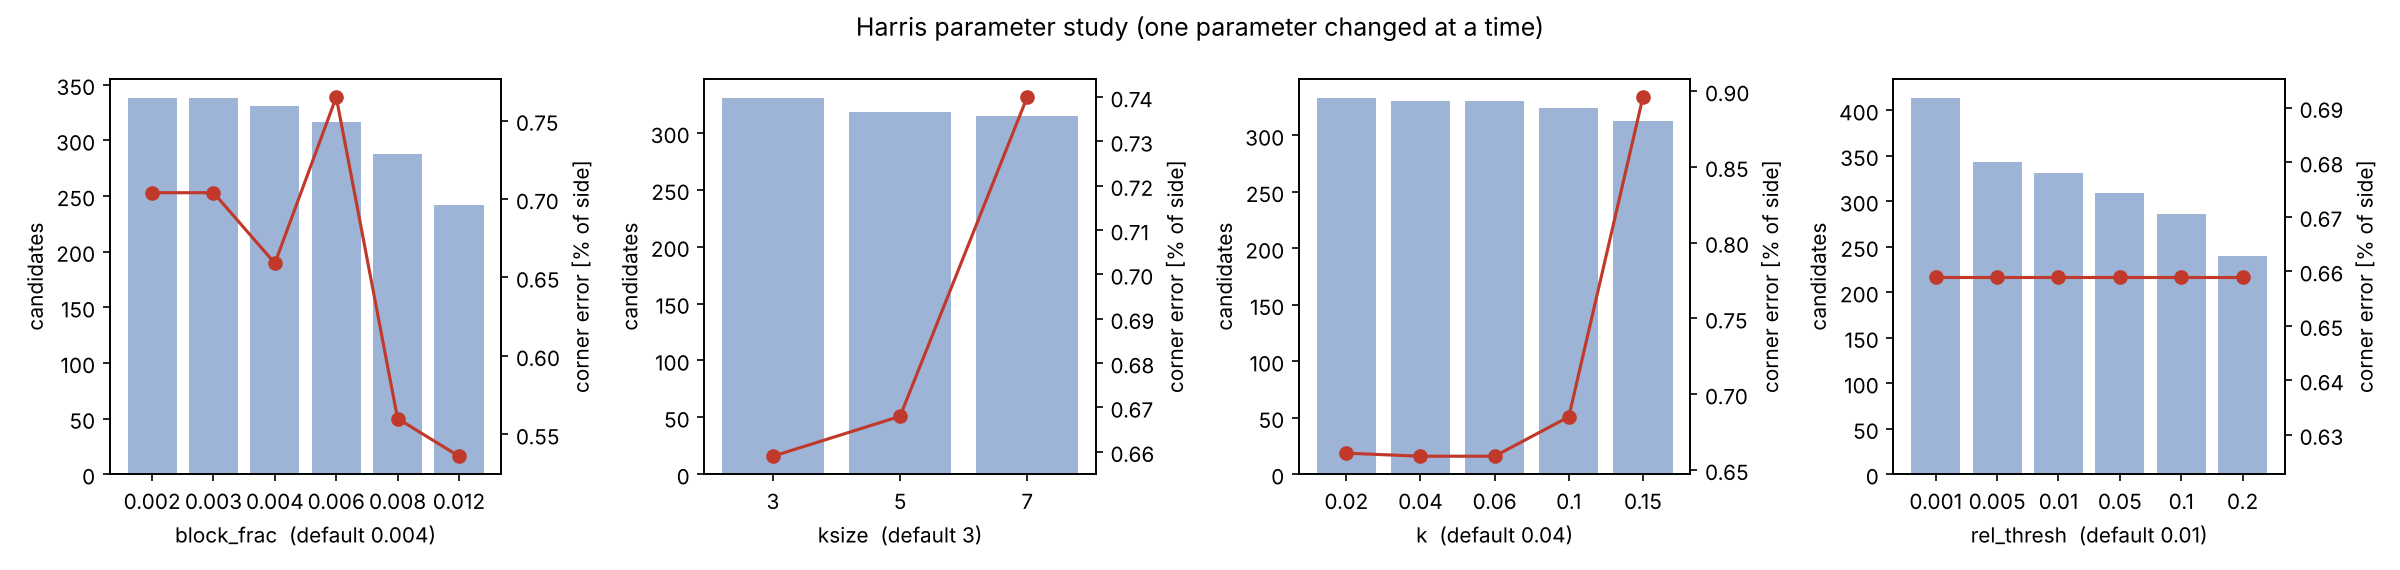
\includegraphics[width=\textwidth]{params.png}
\caption{Parameter study: candidates (bars) and median corner error (line).}
\label{fig:params}
\end{figure*}

%=====================================================================
\section{Rectification}
The corners are mapped to $(0,0),(450,0),(450,450),(0,450)$.

\textbf{Degrees of freedom.} An affine map $[\,a\;b\;t_x;\,c\;d\;t_y\,]$ has
six unknowns; every point pair gives two equations ($x$ and $y$), so three
non-collinear pairs determine it exactly (A3, \texttt{getAffineTransform}
from TL, TR, BL). A homography is a $3\times3$ matrix defined only up to
scale ($H$ and $\lambda H$ give the same mapping), so it has $9-1=8$ unknowns
and needs four pairs (H4, \texttt{getPerspectiveTransform}). A4 fits the
six affine parameters to all four pairs by least squares
(\texttt{estimateAffine2D} with a very large RANSAC threshold so that all
points are inliers and the final refinement is a least-squares fit).

\textbf{What each model can represent.} An affine map keeps parallel lines
parallel and keeps ratios of lengths along a line, so it can only produce
parallelograms. A perspective view of a square is a general quadrilateral
whose opposite sides meet at vanishing points; only the homography (with a
non-zero bottom row $h_{31},h_{32}$) can map the vanishing points back to
infinity.

\textbf{Residuals.} H4 maps all four corners exactly (maximum error
$9\times10^{-6}$\,px over all images). A3 completes the parallelogram from
TL, TR and BL, so the unused BR lands at
$\mathrm{TR}+\mathrm{BL}-\mathrm{TL}$ in the source. In the target image
it lands at $(449.4, 449.3)$ for the frontal IMG\_0836 (1.0\,px from
$(450,450)$), at $(428.8, 462.9)$ for IMG\_0845 (24.8\,px), at
$(376.1, 449.0)$ for IMG\_0838 (73.9\,px) and at $(504.4, 626.3)$ for
IMG\_0842 (184.5\,px), far outside the target square. The landing point is
also written to every result file (\texttt{a3\_br\_mapped}). The A4 RMS residual grows from
0.2 to 36\,px (Table~\ref{tab:stage4}).

%=====================================================================
\section{Affine versus homography}
\textbf{Obliqueness} is defined from the detected quadrilateral as
$o=\max(1-\tfrac{\min(\text{top},\text{bottom})}{\max(\text{top},\text{bottom})},\;
1-\tfrac{\min(\text{left},\text{right})}{\max(\text{left},\text{right})})$:
0 for a parallelogram (no keystone), growing with perspective.
All 13 personal images (obliqueness 0.002--0.27) are used.

\textbf{Measures.} (1) Corner residual: A3 fourth-corner error and A4 RMS.
(2) Grid-line error: I use \texttt{find\_peaks} to detect grid lines from the
horizontal and vertical ink profiles, with a threshold based on the profile's
mean and standard deviation. I match each ideal line position to the nearest
detected peak within 25 pixels and assign a 50-pixel penalty when no line is
found. For border lines, I use a separate threshold based on the profile's
median because these lines may be partially cut off. I also divide the image
into three strips and measure how much each line's position changes between
them to estimate bending.
(3) Recognition: the same OCR stage is run on A3, A4 and H4.

\begin{figure*}[t]
\centering
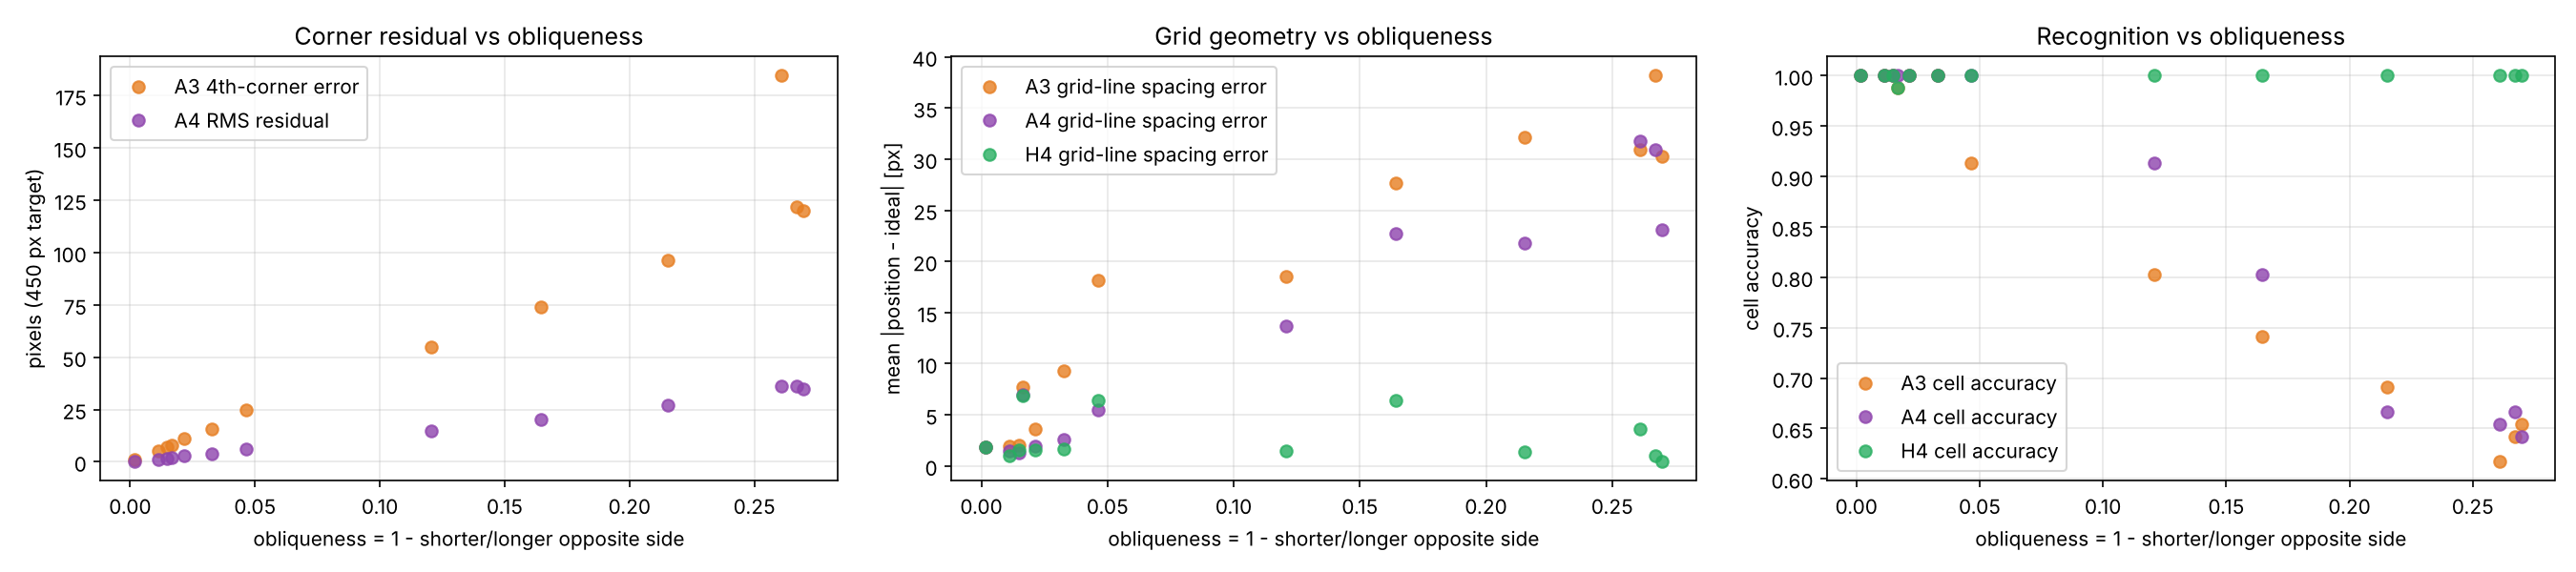
\includegraphics[width=\textwidth]{stage4.png}
\caption{Stage 4 on 13 personal images: corner residual, grid-line spacing
error and cell accuracy against obliqueness.}
\label{fig:stage4}
\end{figure*}

\begin{table}[t]
\centering
\caption{Affine versus homography (detected corners). Residuals and line
spacing error in px of the 450\,px target; accuracy in \%.}
\label{tab:stage4}
\small
\setlength{\tabcolsep}{3pt}
\begin{tabular}{lrrrrrrrr}
\toprule
Image & $o$ & A3 err & A4 rms & \multicolumn{3}{c}{spacing A3/A4/H4} & \multicolumn{2}{c}{acc A3/A4} \\
\midrule
0836 & .002 & 1.0 & 0.2 & 1.8 & 1.9 & 1.8 & 100 & 100 \\
0834 & .022 & 11.3 & 2.8 & 3.6 & 1.9 & 1.6 & 100 & 100 \\
0846 & .033 & 15.8 & 4.0 & 9.3 & 2.5 & 1.7 & 100 & 100 \\
0845 & .046 & 24.8 & 6.3 & 18.1 & 5.5 & 6.4 & 91.4 & 100 \\
0837 & .121 & 54.7 & 14.7 & 18.5 & 13.7 & 1.5 & 80.2 & 91.4 \\
0838 & .164 & 73.9 & 20.1 & 27.6 & 22.7 & 6.4 & 74.1 & 80.2 \\
0839 & .215 & 96.5 & 27.2 & 32.1 & 21.8 & 1.4 & 69.1 & 66.7 \\
0842 & .261 & 184.5 & 36.2 & 30.9 & 31.8 & 3.6 & 61.7 & 65.4 \\
0841 & .270 & 120.1 & 34.9 & 30.3 & 23.1 & 0.5 & 65.4 & 64.2 \\
\midrule
\multicolumn{4}{l}{Mean over 13 images} & 17.1 & 12.7 & 2.7 & 85.0 & 87.3 \\
\bottomrule
\end{tabular}
\end{table}

\textbf{Results.} (Fig.~\ref{fig:stage4}, Table~\ref{tab:stage4}.)
As the obliqueness increases, the errors of A3 and A4 also increase.
H4 gives the lowest average grid-line error at 2.7 pixels, compared with 17.1
pixels for A3 and 12.7 pixels for A4. Although H4 usually has a small error, it
reaches around 6.4--6.9 pixels in IMG\_0835, IMG\_0838, and IMG\_0845. This
happens because the detected Harris corners sometimes lie on the outer edge of
the thick Sudoku border, causing the last grid line to fall outside the
rectified image and receive a 50-pixel missing-line penalty. The error of A3 is about
four times larger than A4 because A3 uses only three corners and estimates the
fourth corner, while A4 uses all four corners and spreads the error over them.
The cell accuracy of A3 first drops below 100\% at 0.046 obliqueness. At the
same obliqueness, A4 still has 100\% accuracy, but its accuracy drops to
91.4\% at 0.12. In highly oblique images, A3 and A4 accuracy drops to around
62--69\%, while H4 stays at 98.8--100\% in all tested images. In the
side-by-side image (Fig.~\ref{fig:sidebyside}), the Sudoku grid lines are
shifted in A3 and A4, while H4 aligns almost perfectly with the green grid
lines.

\begin{figure}[t]
\centering
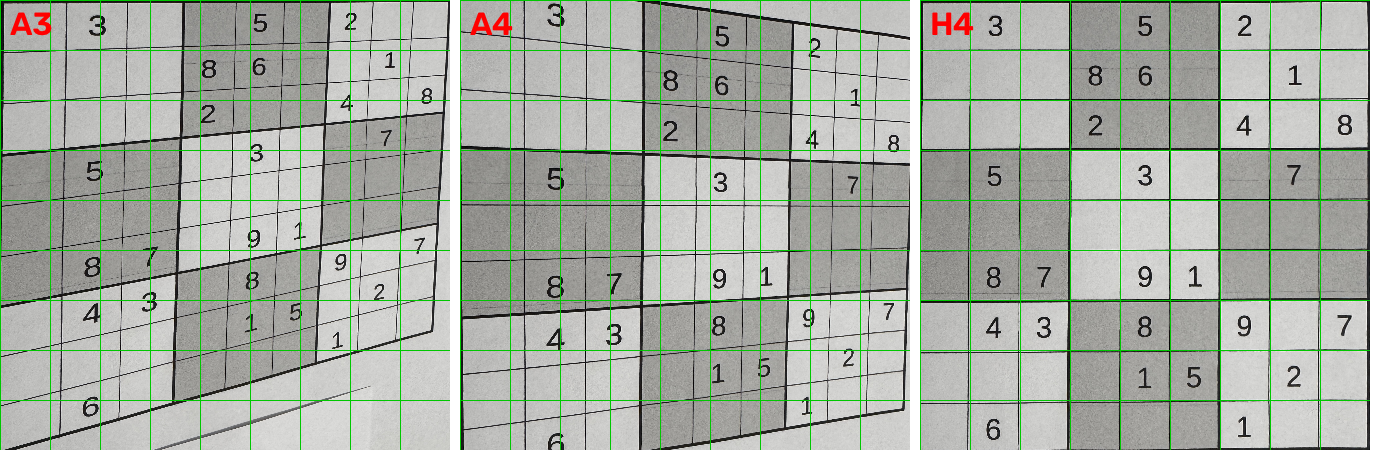
\includegraphics[width=\linewidth]{side_by_side.png}
\caption{Most oblique image (IMG\_0841, $o=0.27$): A3, A4, H4 with the ideal
grid in green.}
\label{fig:sidebyside}
\end{figure}

\textbf{Conclusion and weak perspective.} Affine transformation keeps
parallel lines parallel, so it cannot fully correct perspective distortion.
Affine has 6 degrees of freedom, while homography has 8 degrees of freedom and
can transform non-parallel lines into parallel lines, allowing it to correct a
trapezoid into a square. The weak perspective assumption means that the depth
variation is much smaller than the distance from the camera
($\Delta Z \ll Z$). This happens when the phone is held far from the Sudoku and
almost directly above it. Based on my results, affine transformation can be
acceptable for small obliqueness, approximately up to 0.05, and A4 is more
reliable than A3. For more oblique images, H4 should be used because it gives
more accurate and stable results.

%=====================================================================
\section{Recognition}
\textbf{Margin.} The H4 image is divided into 81 cells of 50\,px. A margin of
10\% (5\,px) is removed on every side: grid lines are 2--6\,px thick in the
rectified image and the rectification can be off by 1--2\,px, while printed
digits occupy the middle $\sim$60\% of a cell. Line pieces that still enter a
cell are removed as connected components: a blob is discarded if it is a long
thin line, or if it touches the crop border and either lies off-centre or
spans more than 80\% of the cell (an L-shaped frame remnant, Sec.~\ref{sec:fail}).

\textbf{Empty-cell criterion (before OCR).} The rectified image is
illumination-normalised and thresholded (adaptive, and darker than 210 on the
normalised scale, then a $2\times2$ opening against sensor noise). A cell is
\emph{filled} if its largest remaining blob covers $\ge2.5\%$ of the cropped
cell and is at least 30\% of its height. Empty-cell F1 is 1.000 on the
personal set.

\textbf{OCR configuration.} Tesseract 5 with
\texttt{--oem 1 --psm 10 -c tessedit\_char\_whitelist=123456789}; if nothing
is returned, \texttt{--psm 13} is tried, then the cell is prepared again at a
larger size. On 362 prepared digits of the personal set (one pass, no
fallback), psm 10 (single character) and psm 7 (single line) read 100\%,
psm 6 (block) 92.8\%, psm 8 (word) and 13 (raw line) 90.1\%; psm 10 matches
the task best. During development, a 24\,px digit height read 98.7\% of 224
synthetic digits versus 89--96\% at 48\,px, so 24\,px was chosen.

\textbf{Cell preparation.} The cleaned binary mask is used only to locate the
digit and erase everything else; the \emph{grey levels} of the normalised cell
are kept, because hard binarisation broke thin strokes on oblique images
(an 8 became ``$||$''). The digit is cropped, contrast-stretched, scaled to
24\,px height and centred on a white $48\times48$ canvas.
\textbf{Effect:} with annotated corners, OCR on the raw $50\times50$ grey cells reaches
85.4\% cell accuracy (13 images), with preparation 100\%. Raw cells fail
because grid-line pieces are read as 1 or 7 and empty cells produce digits.

\textbf{Confusions.} The only error on the personal set is a 1 read as 4 in a
shaded box (F1, Fig.~\ref{fig:fail}).

%=====================================================================
\section{Results}
The development set mentioned in Section 4.1 of the assignment was not
available on the LMS, so we report the personal dataset and, separately, a
held-out synthetic set. The personal dataset has 13 original iPhone
photographs (EXIF kept) of three printed puzzles with different fonts and grid
styles (serif/heavy frame, sans-serif with shaded boxes, monospace with a very
thick frame), each with a handwritten card. Corners were clicked by hand; the
grids come from the printed puzzles. Runtime is 3--6\,s per image on a CPU.

\begin{table}[t]
\centering
\caption{Section 7 metrics on the personal dataset.}
\label{tab:results}
\small
\setlength{\tabcolsep}{4pt}
\begin{tabular}{lrrrrrr}
\toprule
Cond. & $n$ & Corner & Cell acc & F1 & Exact & Robust \\
\midrule
All & 13 & 0.71\% & 99.9\% & 1.000 & 92.3\% & 100\% \\
C1 & 3 & 0.93\% & 99.6\% & 1.000 & 66.7\% & 100\% \\
C2 & 6 & 0.65\% & 100\% & 1.000 & 100\% & 100\% \\
C3 & 2 & 0.55\% & 100\% & 1.000 & 100\% & 100\% \\
C4 & 2 & 0.83\% & 100\% & 1.000 & 100\% & 100\% \\
C5 & 2 & 0.57\% & 100\% & 1.000 & 100\% & 100\% \\
\midrule
Synth.$^\ast$ & 30 & \SYNCORNER\% & \SYNACC\% & \SYNFONE & \SYNEXACT\% & \SYNROB\% \\
\bottomrule
\end{tabular}\\[2pt]
\footnotesize $^\ast$Synthetic images with exact ground truth, never used for tuning.
\end{table}

Part of the residual corner error (about 0.5--1\%) is annotation noise: the
corners were clicked on a downscaled view, where one screen pixel is about
4\,px of a 12\,MP photograph. Four photographs show the page upside down and
are handled by the orientation check (B4).

\textbf{Bonus.} B1: a backtracking solver (most-constrained cell first) solves
the puzzles in 2--13\,ms and checks uniqueness by searching for a second
solution. B2: the solution is drawn in the $450\times450$ frame and mapped
back with $H_4^{-1}$. B3: the 100 grid intersections predicted by $H_4^{-1}$
are matched to Harris candidates, refined with \texttt{cornerSubPix} and fed to
\texttt{findHomography}+RANSAC (68--100 inliers of 100). With the grid-line
measure of Section~IV, the mean error drops from 2.72\,px (H4) to 1.47\,px; it
is lower on 10 of 13 images (largest gain IMG\_0835: 6.9 to 1.1\,px), because
errors of single corners are averaged out, equal on one, and higher on two
(IMG\_0841: 0.45 to 3.15\,px, where a border line is lost). B4: tested by rotating three photographs by
$90^\circ$, $180^\circ$ and $270^\circ$: 12/12 correct.

%=====================================================================
\section{Failure analysis}\label{sec:fail}
\begin{figure}[t]
\centering
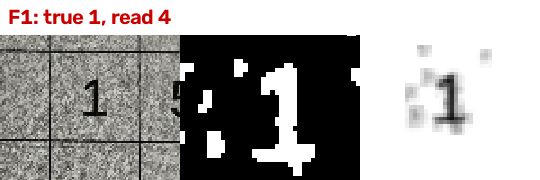
\includegraphics[width=\linewidth]{F1_halftone.png}\\[2pt]
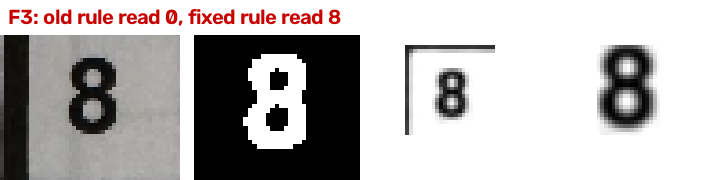
\includegraphics[width=\linewidth]{F3_frame_remnant.png}\\[2pt]
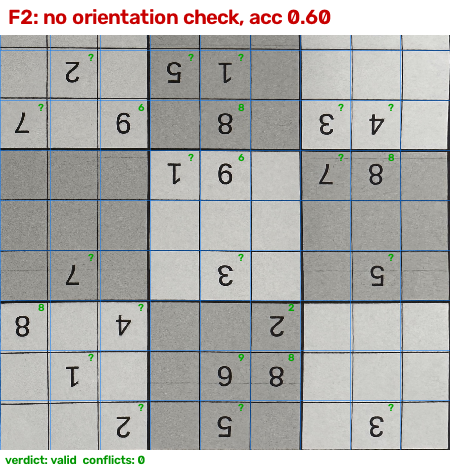
\includegraphics[width=0.49\linewidth]{F2_upside_down.png}\hfill
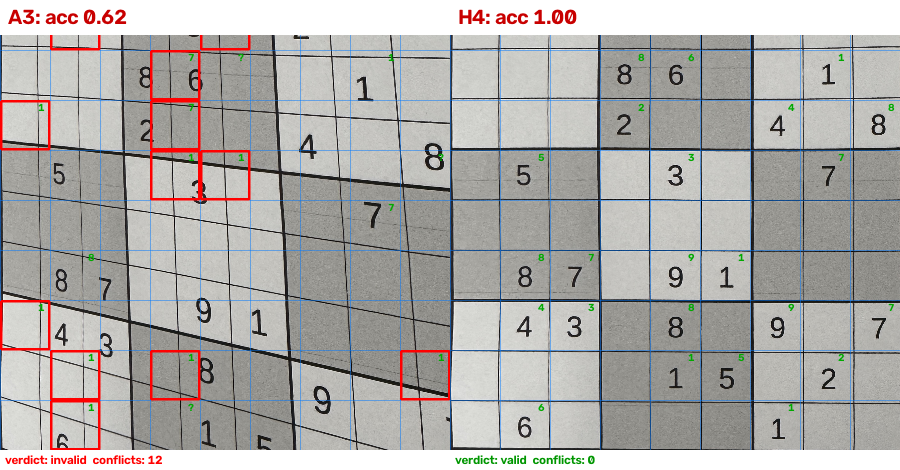
\includegraphics[width=0.49\linewidth,trim=0 0 450 0,clip]{F4_affine_oblique.png}
\caption{Failure cases. Top: F1 (cell, ink mask, OCR input). Middle: F3
(cell, ink, OCR input with the old and the fixed cleaning rule). Bottom left:
F2, upside-down page without orientation check; bottom right: F4, A3
rectification of IMG\_0842 (recognised digit at the top right of each cell,
conflicts in red).}
\label{fig:fail}
\end{figure}

\textbf{F1 -- OCR, halftone grain (IMG\_0835).} The grey box was printed as a
halftone that appears as coarse grain in the photograph. The threshold keeps
grain blobs next to the ``1'' and Tesseract reads 4. Failing stage:
recognition (cell cleaning). A fix would be a size filter relative to the
largest blob or a median filter on shaded cells.

\textbf{F2 -- Corner order, upside-down page (IMG\_0842).} Without the
orientation check the corners are geometrically correct but in the wrong
order; the rectified image is upside down and only 60\% of the cells are
right. Notably the validity check still says \emph{valid}: an upside-down
6/9 or 1 forms no conflict. Failing stage: corner selection (the diagonal
rule only knows image directions). Fixed by the OCR-confidence orientation
check.

\textbf{F3 -- Cell cleaning, frame remnant.} In an early photograph the thick
outer frame left an L-shaped piece in the corner cell; its centre was near the
cell centre, so the old ``touches border and off-centre'' rule kept it and the
8 was read as 3. Failing stage: cell extraction. Fixed by also discarding
border-touching blobs that span more than 80\% of the cell.

\textbf{F4 -- Affine model at strong obliqueness (IMG\_0842, $o=0.26$).} A3
leaves curved-looking, non-parallel grid lines that cross cell boundaries;
digits fall into neighbouring cells, 62\% accuracy and 12 conflicts. H4 reads
100\%. Failing stage: rectification model (Stage 4).

\textbf{F5 -- Very oblique, low-resolution input (synthetic).} On a 1600\,px
synthetic image at $50^\circ$ tilt the far rows are only $\sim$25\,px high
before rectification; after warping they are blurred and 10 digits are not read
(85.2\% cell accuracy). Failing stage: recognition, caused by
the loss of resolution in the far part of the image.

%=====================================================================
\section{Conclusion and limitations}
Restricting Harris candidates to a grid-like region and taking diagonal
extreme points gives sub-1\% corner errors on clutter, rotation, shadow and
strong perspective. The comparison shows that affine rectification is only
acceptable for near-frontal views ($o\lesssim0.05$), consistent with the weak
perspective assumption $\Delta Z\ll\bar Z$; the homography is required
otherwise. Limitations: the personal set is small (13 images, three puzzles
generated in three styles rather than taken from three publishers); the region
step assumes an unbroken
outer border; rotations near $45^\circ$ are ambiguous for the diagonal rule;
halftone shading can still confuse OCR; and the development set was not
available for an independent check.

\clearpage
\onecolumn
\appendix
\section*{Appendix C. AI-use disclosure}
\begin{center}
\small
\begin{tabular}{p{2.2cm}p{3.6cm}p{5cm}p{5cm}}
\toprule
Tool & Purpose / stage & What I asked (summary) & What I kept, changed or rejected \\
\midrule
Claude (Anthropic) & All stages 1--6 except the Stage 2 region finder and corner selection (\texttt{my\_region.py}, \texttt{my\_corners.py}) and the Stage 4 measures (\texttt{my\_stage4.py}); bonus B1--B4; analysis and plotting scripts (parameter study, Stage 4 comparison tool, OCR study, evaluation); annotation tool & To write the pipeline and analysis code in a simple, readable style, and to debug it on my photographs (e.g.\ the L-shaped frame remnant, the upside-down pages) & \STUDENTKEPT \\
Claude (Anthropic) & Printable test puzzles, synthetic test images & To generate three puzzles in different styles and synthetic photographs with known ground truth & Printed and photographed the puzzles myself; synthetic images used for testing only \\
Claude (Anthropic) & Report, except the Stage 2 corner-selection rule text and the Stage 4 Measures, Results and Conclusion paragraphs & To draft the report text from my results and figures & \STUDENTREPORT \\
Claude (Anthropic) & Learning and feedback for Stage 2 and Stage 4 (\texttt{my\_region.py}, \texttt{my\_corners.py}, \texttt{my\_stage4.py}, Stage 4 paragraphs) & Explanations of Harris parameters, degrees of freedom, weak perspective; step-by-step questions; running and testing my code on my photographs, putting it into the project, and pointing out errors (e.g.\ the A4 line-matching error and the border threshold) & I kept the ideas that worked, changed the grid scoring method to detect and count lines, and corrected problems with duplicate peaks, line matching and border thresholds. I used the test results to check my decisions. \\
\bottomrule
\end{tabular}
\end{center}

\noindent My own work: printing and photographing the puzzles, the handwritten
card, clicking the ground-truth corners for all 13 photographs, running the
experiments, \STUDENTOWN. My work also included developing the Stage 2
corner-selection and puzzle-region methods, choosing the thresholds,
implementing the grid-line scoring method, and revising the code after testing.
For Stage 4, I worked on the obliqueness formula, grid-line measurement, and
interpretation of the comparison results. I also reviewed the limitations and
updated the report explanations.


\vspace{0.8cm}
\noindent Name: Furkan Can \hfill Student no.: 042301138 \hfill Signature: \rule{3.5cm}{0.4pt}

\vspace{0.3cm}
\noindent Date: 05.11.2026 (first submission), revised 06.11.2026

\end{document}
